\documentclass[main]{subfiles}

\begin{document}

\chapter{Post Assembly}

\section{Introduction}
% historique



\begin{figure}[ht]
    \subfloat[][A synthetic metagenome of 5 species wis a different coverage]{
        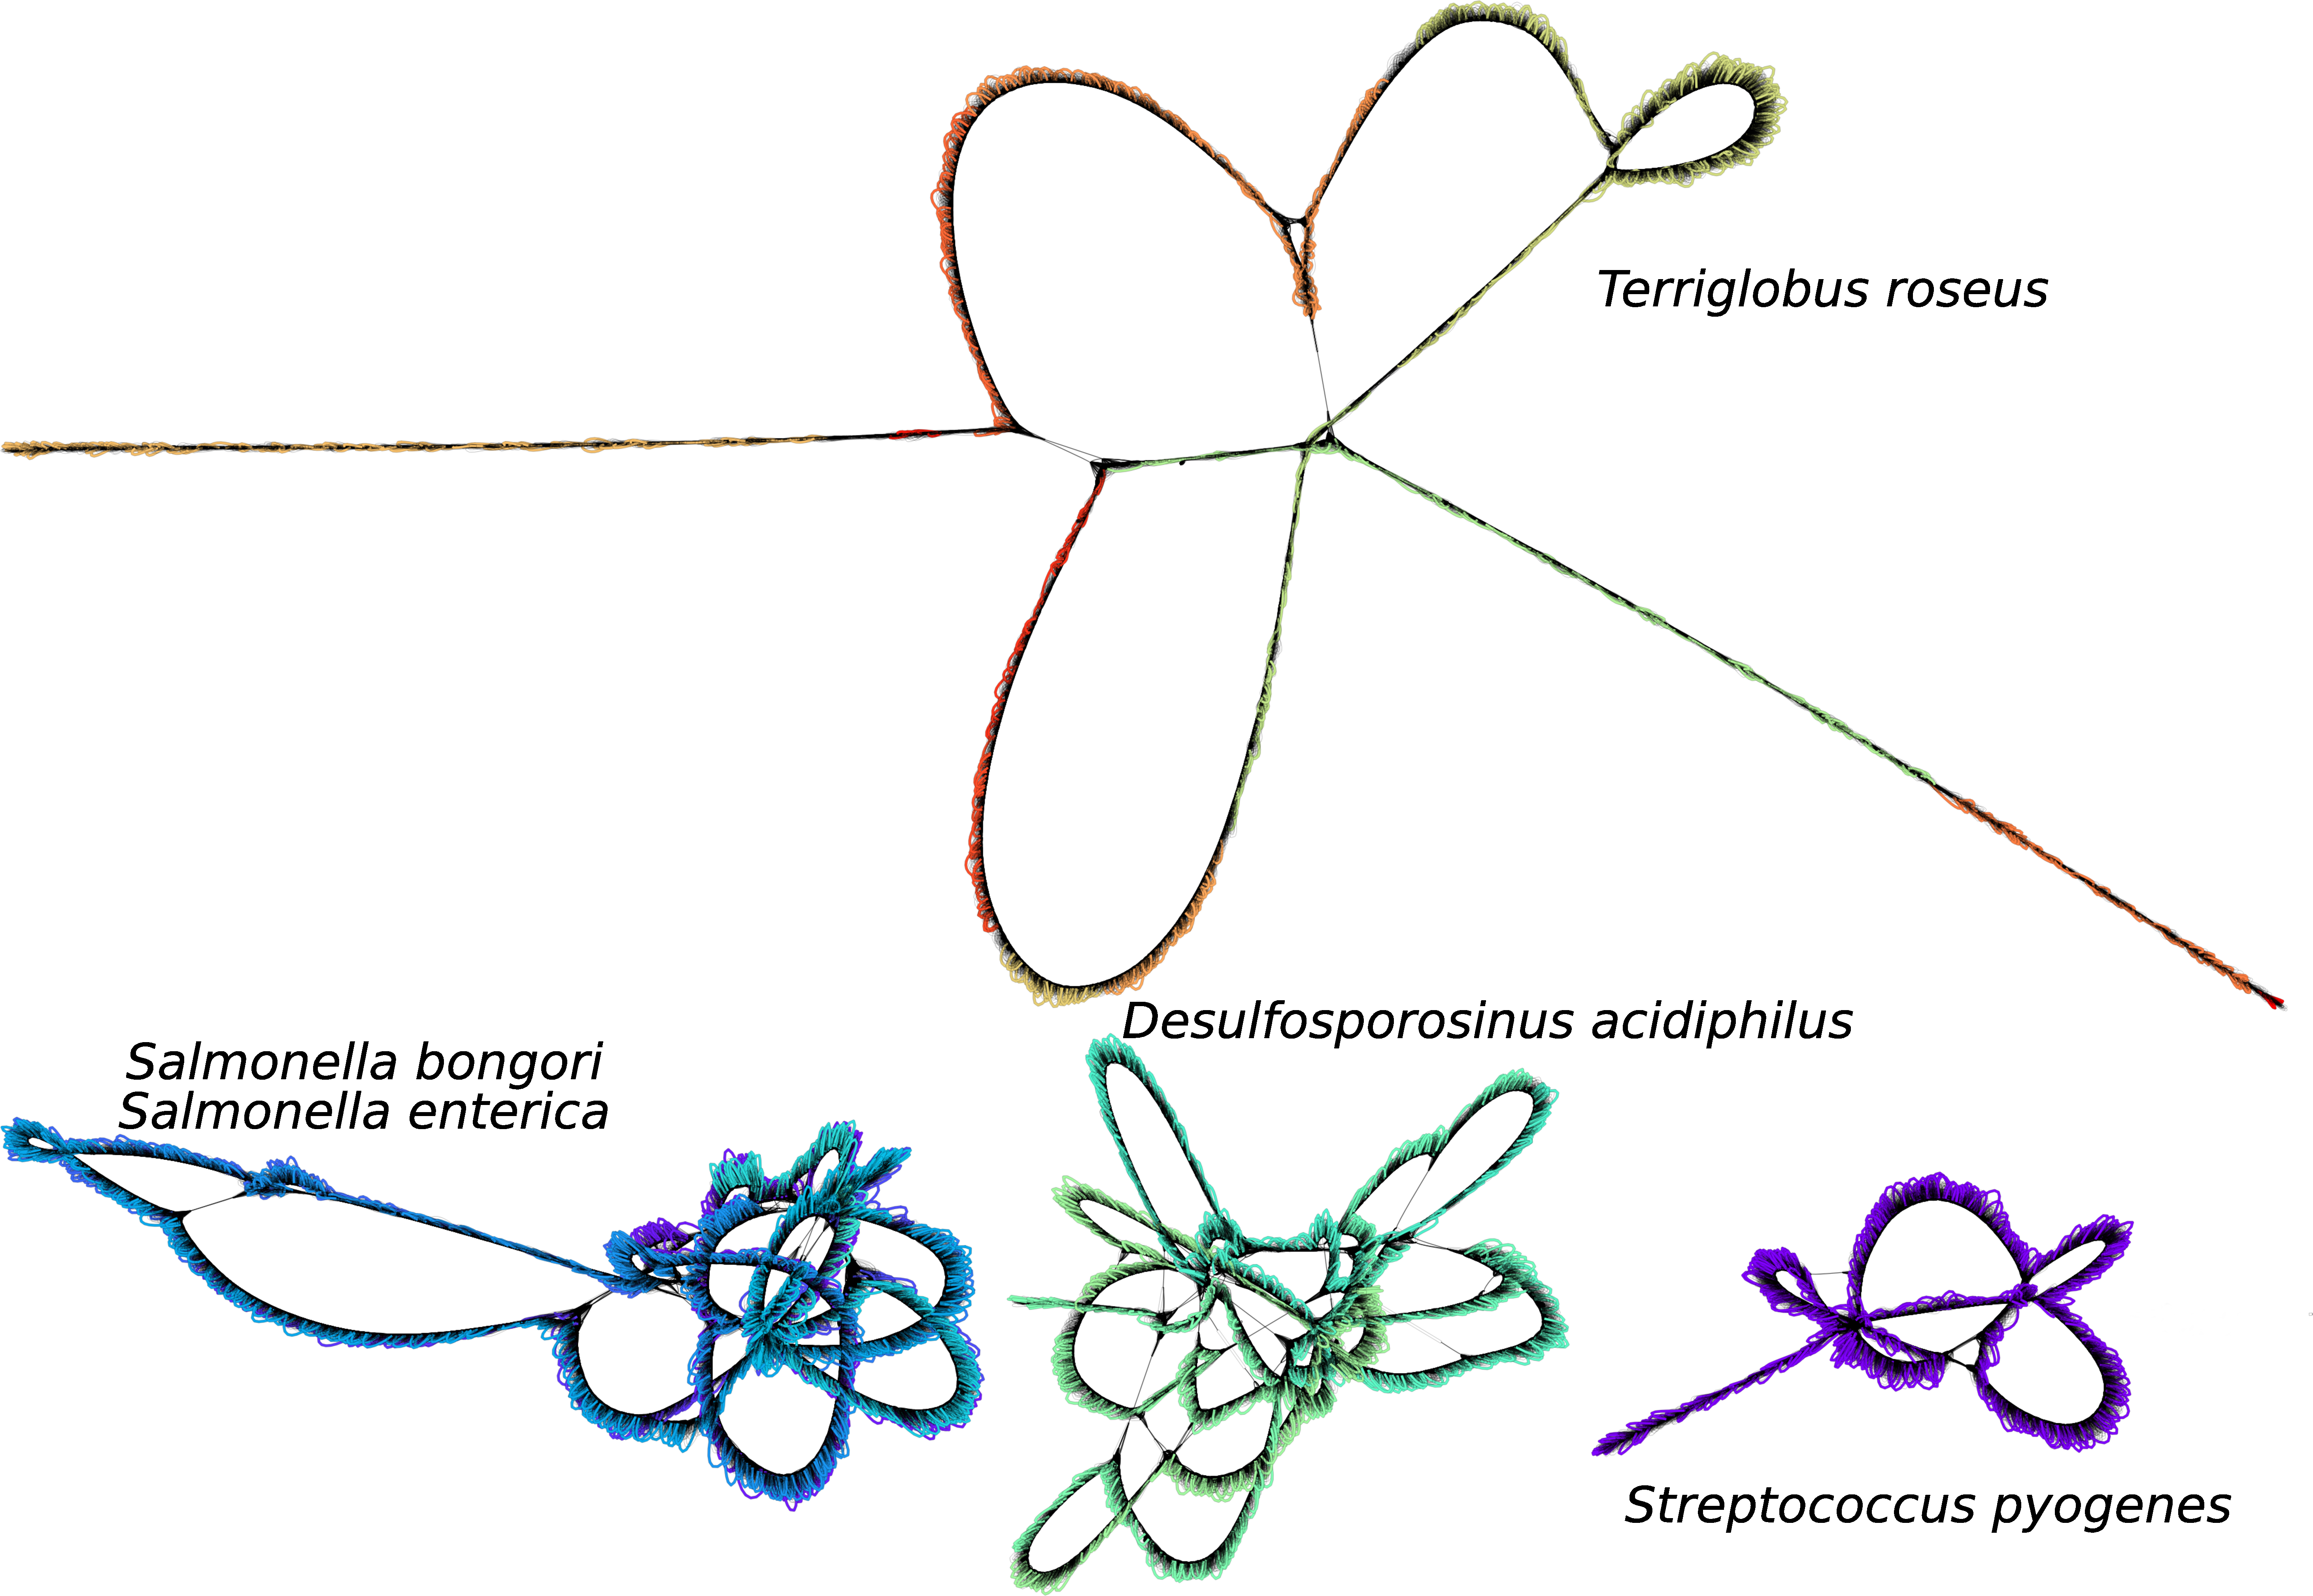
\includegraphics[width=0.9\textwidth]{./postassembly/images/mbrac5_projection.pdf}
        \label{postassembly:fig:intro:mbrac5}
    }
    \newline
    \subfloat[][\textit{Terriglobus roseus} with a 20x coverage]{
        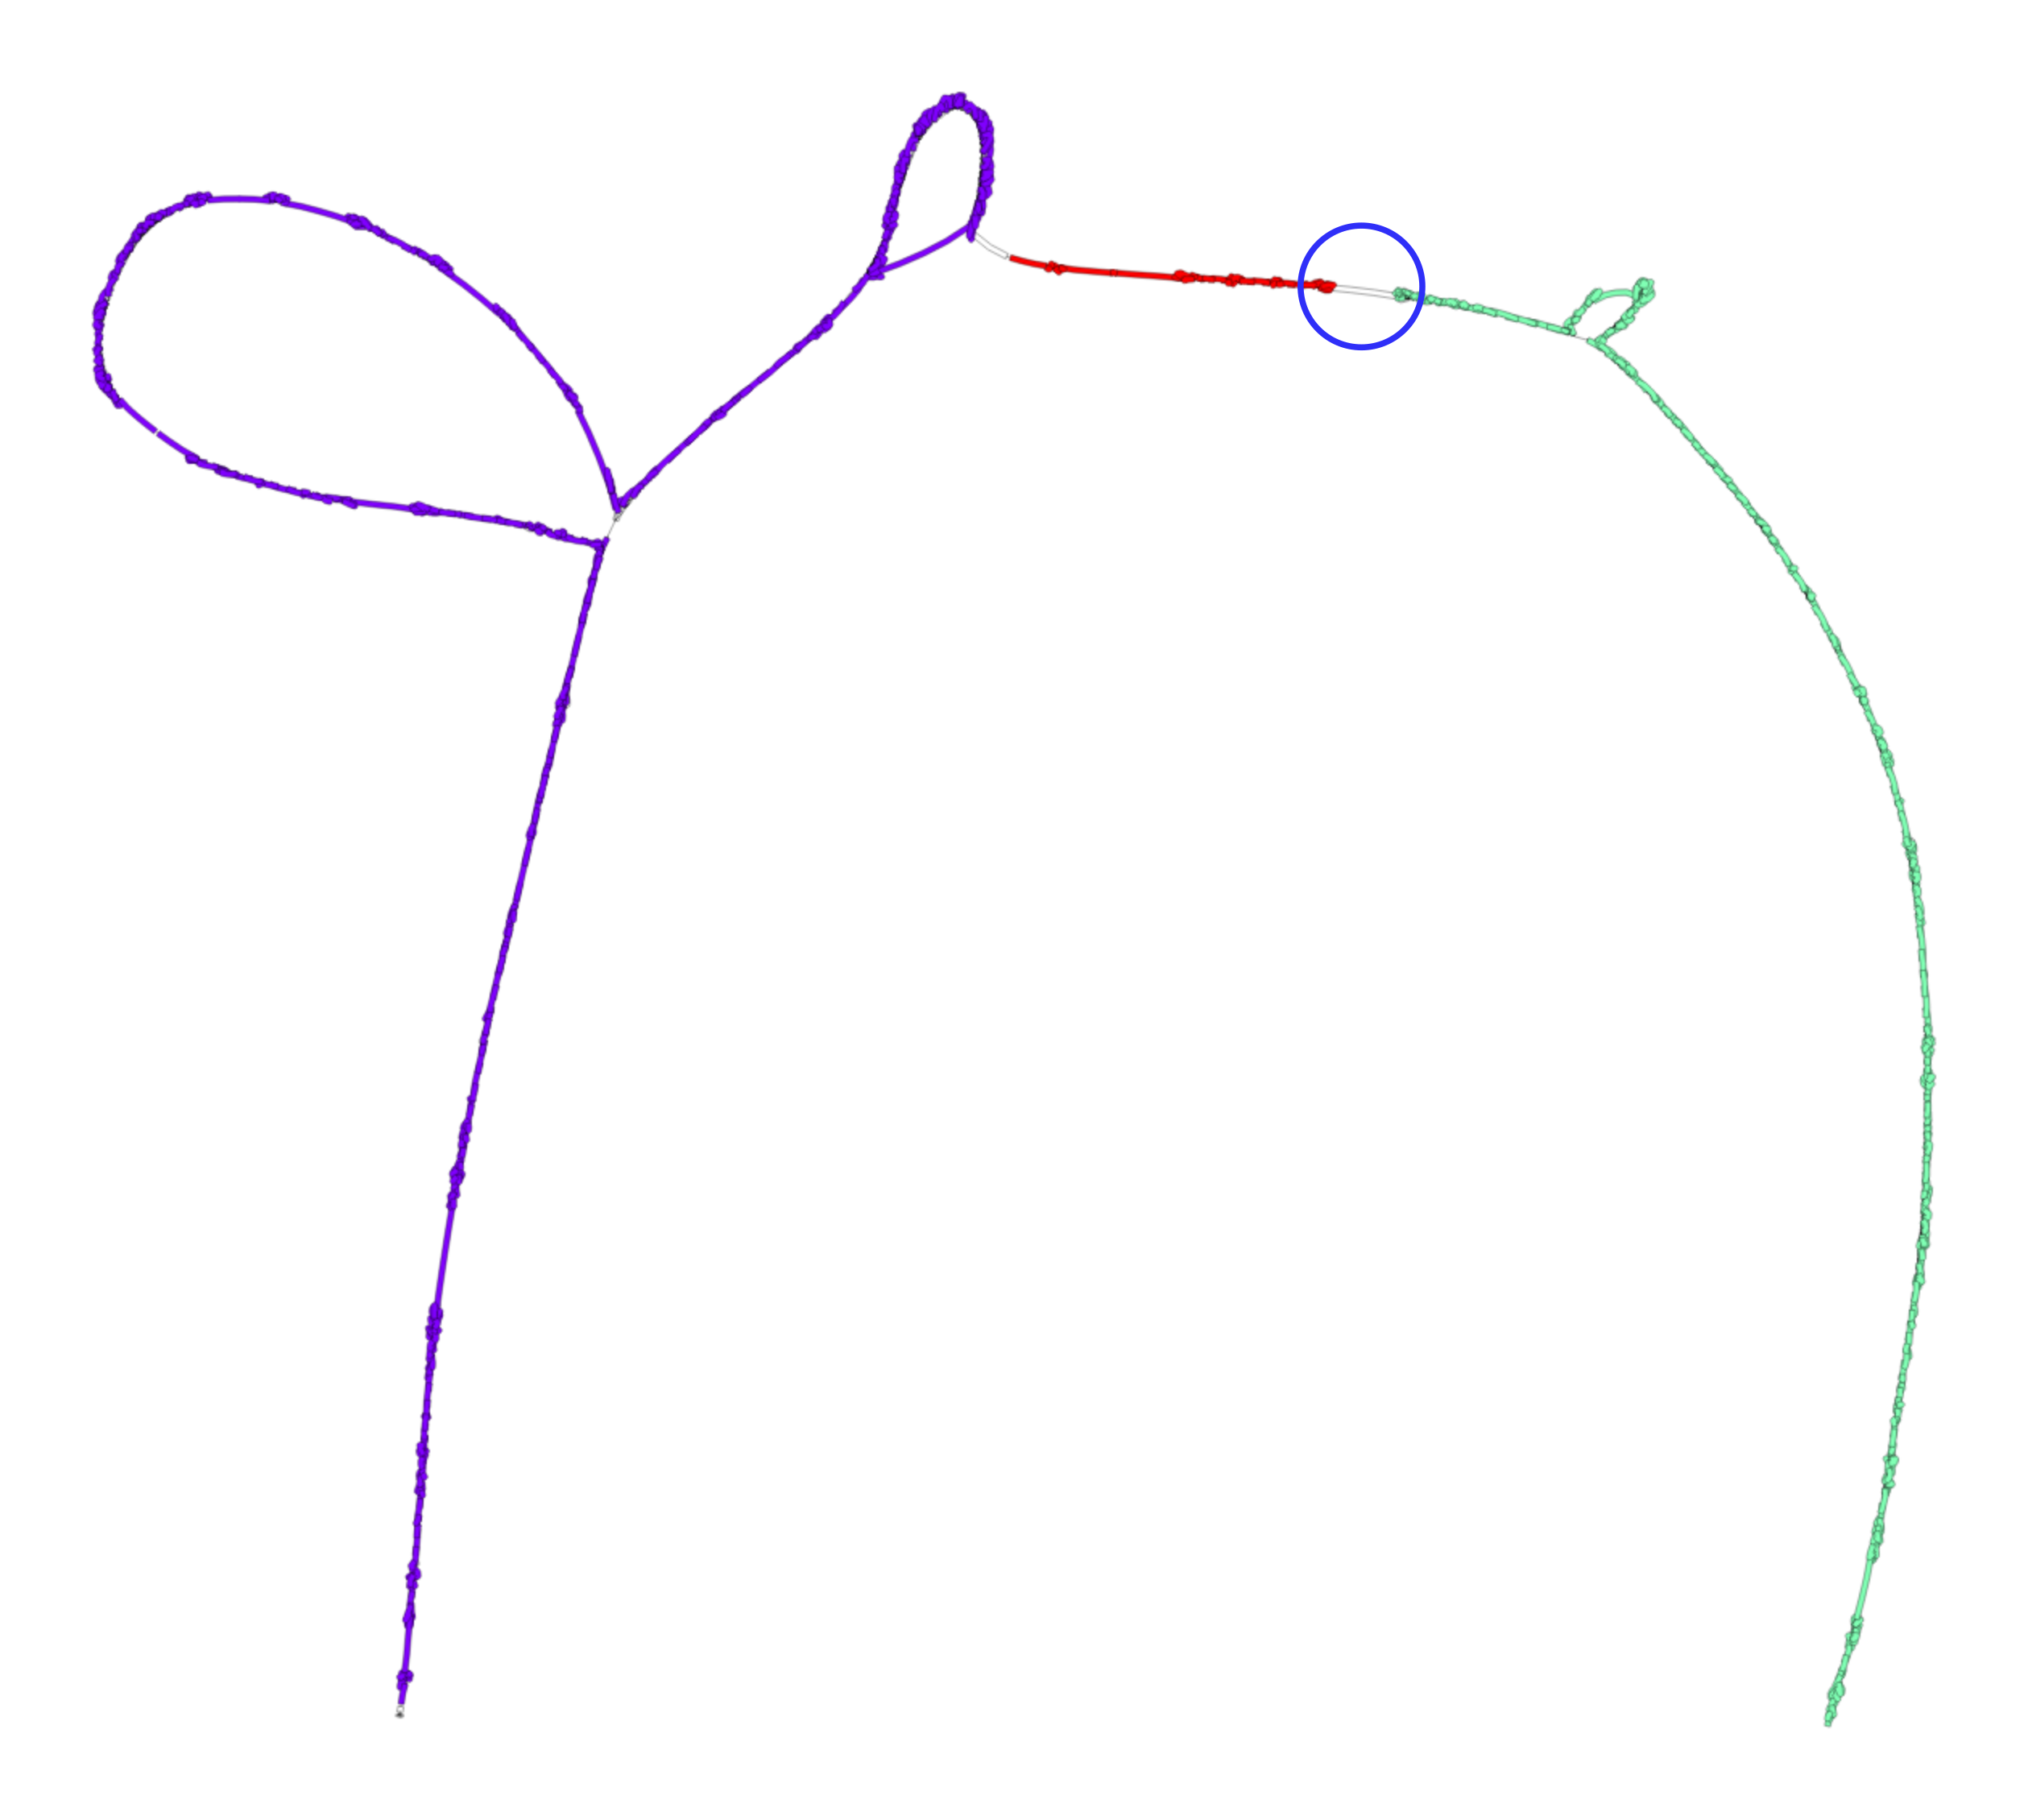
\includegraphics[width=0.9\textwidth]{postassembly/images/t_roseus_projection.png}
        \label{postassembly:fig:intro:troseus}
    }
    \caption{This graph was the overlap graph (found by \minimap), read used by \canu to build a contigs was are colored with same color. We can observe many unexpected fragmentation in (a) and this fragmentation is still be present in genomic context (b)}
    \label{fig:my_label}
\end{figure}

\onlyinsubfile{
\bibliographystyle{plainnat}
\bibliography{postassembly}
\addcontentsline{toc}{chapter}{Bibliography}
}

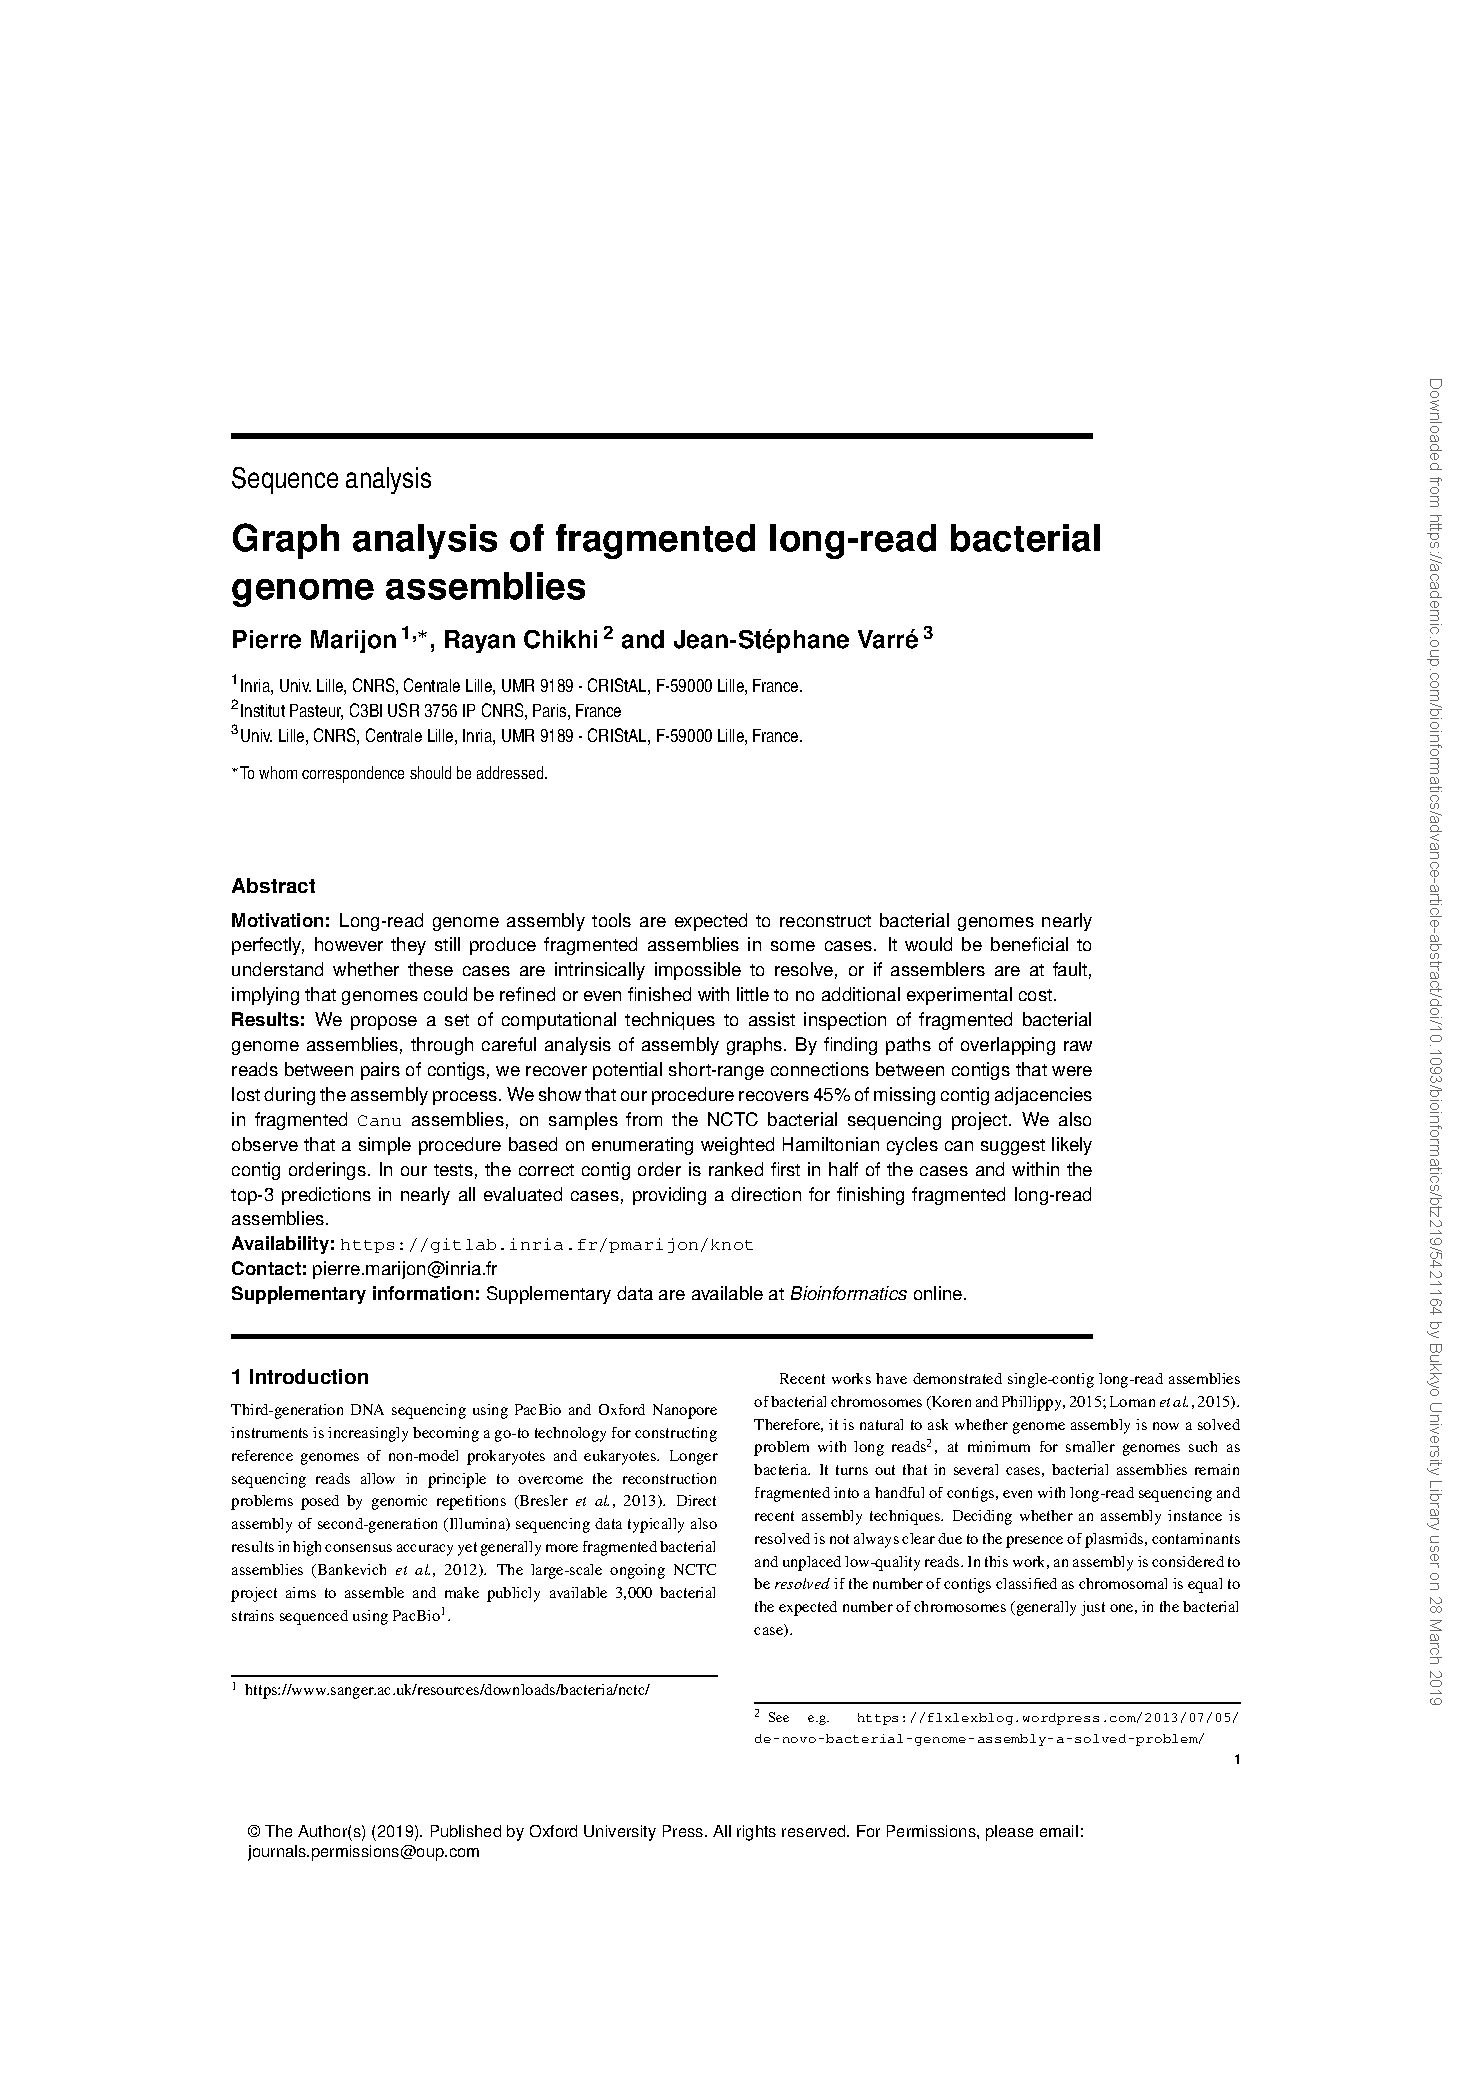
\includepdf[pages=-]{paper/knot.pdf}

\end{document}